
% %NOTE:
% % CHECKED WITH SLIDES: YES!
% % CHECKED WITH EXERCISES: NO -- TODO
% % MISSING: -


\section{Communication}

\subsection{Requirements}
\begin{itemize}[noitemsep]
\item Performance: bandwith, latency, guaranteed behaviour (real-time)
\item efficient: cost (material, installation), low power
\item Robustness: fault tolerance, security, safety, maintainability
\end{itemize}

\subsection{Classification}

\begin{figure}[ht]
	\centering
  	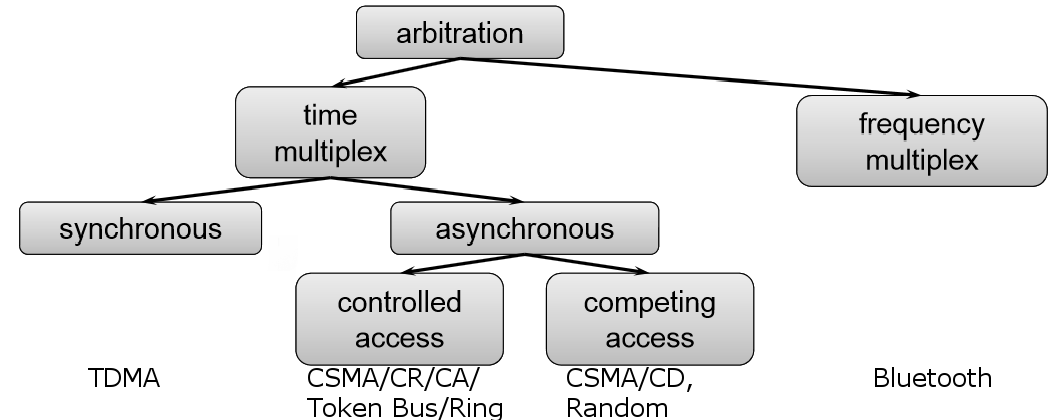
\includegraphics[scale=0.4]{img/8_classification.png}
	\caption{Overview over the communication classifications}
	\label{fig_classification}
\end{figure}


\subsection{Random Access}
\subsubsection{Fully randomized}
no access control; requires low medium utilization, high access conflicts
\subsubsection{Slotted random access}
Start and end of access to the channel at given intervals

\begin{theorem}
Given sending rate $p$ and $n$ stations: probability that a slot is not taken by others is $(1-p)^{n-1}$
\end{theorem}

\begin{theorem}
Given sending rate $p$ and $n$ stations: probability that a station transmits successfully is $p(1-p)^{n-1}$
\end{theorem}

\begin{theorem}
Optimal sending rate $p$ in case of $n$ stations is given by $p= 1/n$
\end{theorem}



\subsection{Time Division Multiple Access - TDMA}

\begin{itemize}[noitemsep]
\item Time multiplex, synchronous
\item Communication in statically allocated time slots
\item Synchronization necessary: master node sends out a synchronization frame or periodic repetition of communication frame
\item Examples: satellite networks
\end{itemize}


\subsection{Carrier Sense Multiple Access / Collision Detection -- CSMA/CD}

\begin{itemize}[noitemsep]
\item Computers connected using a single cable. Only one computer can transmit at a time
\item before starting to transmit, check whether the channel is idle
\item if a collision is detected (several nodes started almost 
simultaneously), wait for some time (backoff timer)
\item Collision detected by invalid CRC or unexpected voltages and currents
\item repeated collisions result in increasing backoff times
\item Examples: Ethernet, IEEE 802.3
\end{itemize}

\begin{definition}[Maximum Distance]
The distance L [m] two nodes are separated from.
\end{definition}

\begin{definition}[Propagation Speed]
Speed $\sigma$ [m/s] the signal travels 
\end{definition}

\begin{definition}[Slot-time]
The minimum time $t_w = \frac{2L}{\sigma}$ [s] a node has to wait to reattempt transmission. Also this is the worst case time needed to detect a collision.
\end{definition}

\begin{definition}[Minimum Packet size]
TODO (wohl data-rate*slot-time)
\end{definition}

\begin{definition}[data-rate]
The rate the data is transmitted from one station to the other: $B$ [bytes/sec].
\end{definition}

\begin{theorem}
Given, that as exponential back-off algorithm in collision m a random value from $K \in \{0, ..., 2^m-1 \}$ is choosen. The probability of $s$ successive collisions is given by: $p_s = \frac{1}{2} *\frac{1}{2^2} * ... * \frac{1}{2^{s-1}} = \frac{1}{2^{ \sum\limits_{i= 1}^{s-1} i} }$, where $\sum\limits_{i = 1}^{s-1} i = \frac{(s-1)*s}{2}$
\end{theorem}

\subsection{Token Protocols}
\begin{itemize}[noitemsep]
\item Token value determines which node is transmitting and/or should transmit next
\item Only the token holder may transmit
\item Null messages with tokens must be passed to prevent network from going idle
\item IEEE 802.4, TokenRing
\end{itemize}

\subsection{Token Ring}
\begin{itemize}[noitemsep]
\item Token owner can send data. Waits for acknowledgement from the receiver
\item Sends null token to the next owner
\end{itemize}

\subsection{Carrier Sense Multiple Access / Collision Avoidance - CSMA/CA - Flexible TDMA (FTDMA)}

\begin{itemize}[noitemsep]
\item reserve s slots for n nodes
\item nodes keep track of global communication state by sensing
\item nodes start transmitting a message only during the assigned slot
\item if $s = n$, no collisions. if $s < n$, statistical collision avoidance
\item examples: 802.11
\end{itemize}



\subsection{Carrier Sense Multiple Access / Collision Resolution -- CSMA/CR}

\begin{itemize}[noitemsep]
\item Before any message transmission, there is a global arbitration
\item Each node is assigned a unique identification number
\item All nodes wishing to transmit compete by transmitting a binary signal based on their identification value
\item A node drops out the competition if it detects a dominant state while transmitting a passive state
\item The node with the lowest identification value wins
\end{itemize}




\subsection{FlexRay}

\subsubsection{General}
\begin{itemize}[noitemsep]
\item By FlexRay consortium (BMW, Ford, Bosch, 
DaimlerChrysler, General Motors, Motorola, Philips)
\item High data rates can be achieved: 10Mbit/sec, but even much higher data rates possible
\end{itemize}

\subsubsection{Principle}
\begin{itemize}[noitemsep]
\item Cycle is subdivided into a static and a dynamic segment
\item Static segment is based on a fixed allocation of time slots to nodes
\item Dynamic segment for transmission of ad-hoc communication with 
variable bandwidth requirements
\item Two independent channels to eliminate single-point failures
\item Star and Bus topologies possible
\end{itemize}

\subsubsection{TDMA}
\begin{itemize}[noitemsep]
\item all static slots are the same length whether used or not
\item all slots are repeated in order every communication cycle
\item slots are lock-stepped in order on both channels
\end{itemize}





\subsubsection{Flexible TDMA}
\begin{itemize}[noitemsep]
\item each minislot is an opportunity to send a message
\item if message isn’t sent, minislot elapses unused (short idle period)
\item all nodes watch whether a message is sent so they can count minislots
\end{itemize}


\subsection{Bluetooth}
\subsubsection{Design Goals}
\begin{itemize}[noitemsep]
\item small size
\item low cost
\item low energy
\item secure transmission, robust transmission
\end{itemize}

\subsubsection{Technical Data}
\begin{itemize}[noitemsep]
\item 2.4 GHz Band
\item 10-100 m transmission range, 1 Mbit/s bandwidth for each connection
\item simultaneous transmission of multimedia streams (synchronous) and data (asynchronous)
\item ad hoc network, no centralized coordination, multi-hop communication
\end{itemize}


\subsubsection{Frequency Hopping}
\begin{itemize}[noitemsep]
\item Transmitter jumps from one frequency to another with a fixed rate (1600 hops/s). The ordering (channel sequence) is determined by a pseudo random sequence of length $2^{27}-1$
\item Frequency range (2402 + k) MHz, k = 0 ...78
\item The data transmission is partitioned into time windows of length 0.625  ms; each packet is transmitted by means of a different frequency
\item For security reasons.
\end{itemize}

\subsubsection{Network Topologies}
Hierarchical structure (scatternet) of small nets (piconet)


Piconet:
\begin{itemize}[noitemsep]
\item A piconet contains 1 master and maximally 7 slaves
\item All nodes in a piconet use the same frequency hopping scheme (channel sequence) which is determined by the device address of the master BD\_ADDR and phase which is determined by the system clock of the master.
\item Connections are either one-to-one or between the master and all slaves (broadcast).
\item A slave can never become active by themselves. Master has to poll!
\end{itemize}

Scatternet
\begin{itemize}[noitemsep]
\item Several piconets with overlapping nodes form a scatternet. Up to 10 piconets per scatternet
\item A node can simultaneously have the roles of slaves in several piconets and the role of a master in at most one piconet.
\item The channel sequences of the different piconets are not synchronized. 
\item As a result, large network structures can emerge and multi-hop communication is possible
\end{itemize}

\subsubsection{Packet Format}
\begin{itemize}[noitemsep]
\item The (channel) access code identifies all packets between Bluetooth devices.
\item Packet Header identifies and characterizes connection between master and slave
\item 126bit MAC-header (Channel Access Code and Packet Header)
\item 24bit used for Payload-Header and CRC
\item A typical packet has therfore a payload of 216 bits (DH1)
\end{itemize}


\begin{figure}[ht]
	\centering
  	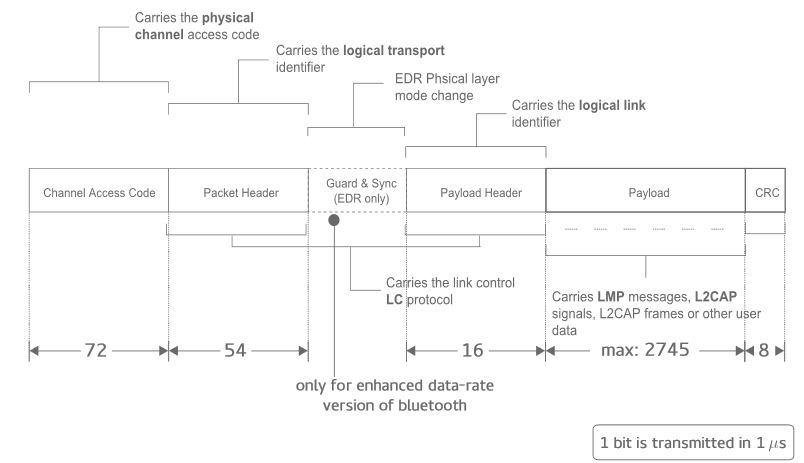
\includegraphics[scale=0.4]{img/8_bluetooth_packet.png}
	\caption{How a bluetooth packet is built up. Numbers in bit}
	\label{fig_bluetooth_packet}
\end{figure}


\subsubsection{Addressing}
\begin{itemize}[noitemsep]
\item Bluetooth Device Address: BD\_ADDR: 48 Bit, unique address for each device
\item Active Member Address AM\_ADDR: 3 Bit for maximally 7 active Slaves in a piconet, address “Null“ is a broadcast to all slaves.
\item Parked Member Address PM\_ADDR: 8 Bit for parked slaves.
\end{itemize}

\subsubsection{Connection Types}
\begin{itemize}[noitemsep]
\item Synchronous Connection-Oriented (SCO)
	\begin{itemize}
	\item Point to point full duplex connection between master and slaves
	\item Reservation-based: Master reserves slots to allow transmission of packets in 
	regular intervals. 
	\end{itemize}
\item Asynchronous Connection-Less (ACL)
	\begin{itemize}
	\item Asynchronous service
	\item No reservation of slots
	\item The master transmits spontaneously, the addressed slave answers in the following interval
	\item Polling required
	\end{itemize}
\end{itemize}

\subsubsection{Frequency Hopping Time Multiplex}
\begin{itemize}[noitemsep]
\item A packet of the master is followed by a slave packet
\item After each packet, the channel (frequency) is switched

\end{itemize}

\subsubsection{Multi-Slot Communication}
\begin{itemize}[noitemsep]
\item Master can only start sending in even slot numbers.
\item Packets from master or slave have length of 1, 3 or 5 slots
\item In total, 2, 4 or 6 slots are used (for answering an additional slot is used)
\item When the slave sends data across multiple slots, the frequency of the tramission is kept the same. The missed frequencies are skipped
\end{itemize}

\begin{figure}[ht]
	\centering
  	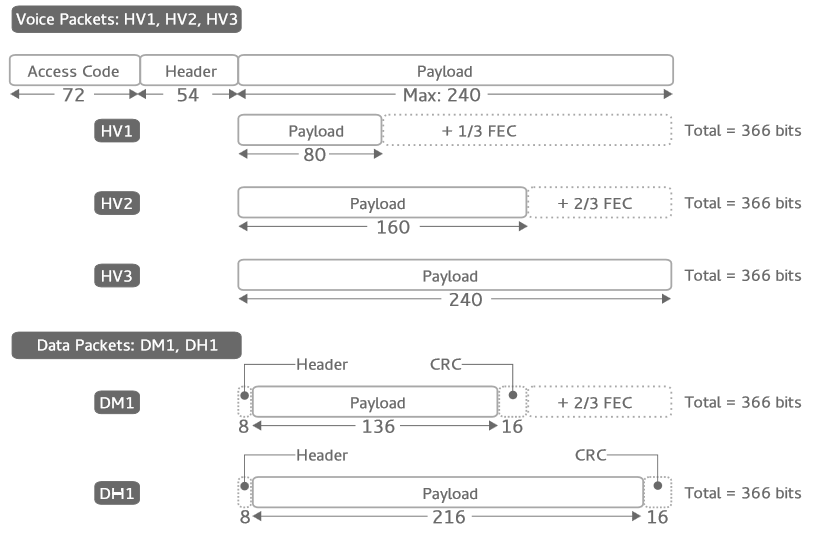
\includegraphics[scale=0.4]{img/8_packet_1.png}
	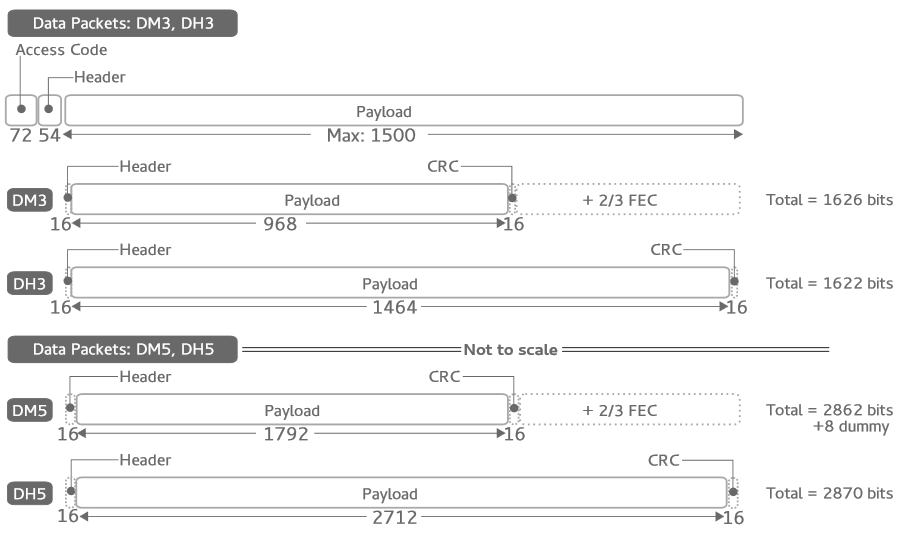
\includegraphics[scale=0.3]{img/8_packet_2.png}
	\label{fig_bluetooth_packet_overview}
\end{figure}


\subsubsection{Modes of Operation}
\begin{itemize}[noitemsep]
\item Inquiry (master identifies addresses of neighboring nodes)
\item Page (master attempts connection to a slave whose address BD\_ADDR is known)
\item Connected (connection between master and slave is established) 
\end{itemize}

\subsubsection{States in Connection Mode}
\begin{itemize}[noitemsep]
\item active (active in a connection to a master)
\item hold (does not process data packets)
\item sniff (awakens in regular time intervals)
\item park (passive, in no connection with master but still synchronized)
\end{itemize}

\subsubsection{Synchronization in Connection Mode}
\begin{itemize}[noitemsep]
\item channel sequence of a piconet is determined by the BD\_ADDR of the master
\item The phase within the sequence is also determined by the master; all slaves follow
\end{itemize}

\begin{figure}[ht]
	\centering
  	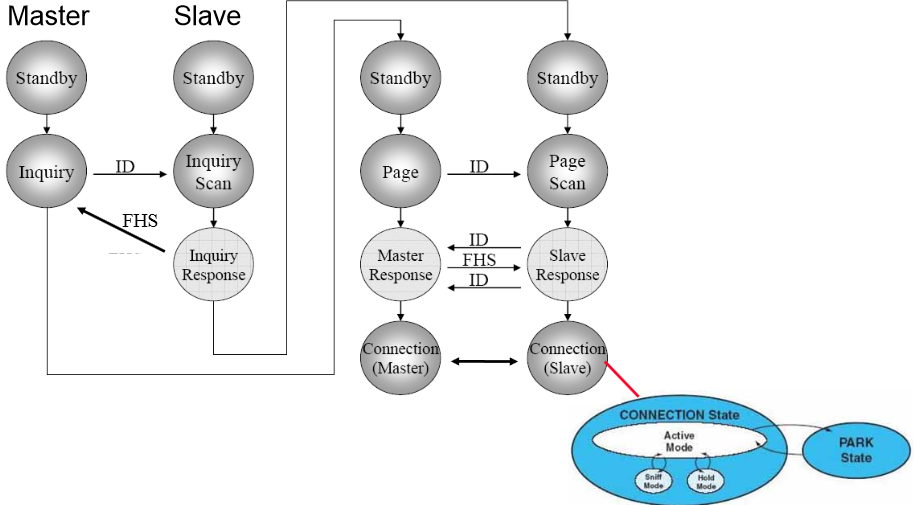
\includegraphics[scale=0.4]{img/8_establish_connection.png}
	\caption{Overview how Bluetooth establishes a connection between Master and Slave}
	\label{fig_establish_connection}
\end{figure}


\subsubsection{Page Mode}
\begin{enumerate}[noitemsep]
\item Page: Master transmits its own and slave address to slave (it uses a special channel sequence)
\item page scan: Slave listens, whether its own address is sent from a master
\item Slave answers the master with its own address
\item Master sends FHS-packet (frequency hop synchronization) to slave. It contains the channel sequence and the phase of the piconet
\end{enumerate}

\subsubsection{Protocol Hierarchy}
\begin{itemize}[noitemsep]
\item baseband specification: defines the packet formats, the physical and logical channels, the error correction, the synchronization between receiver and transmitter, and the different modes of operation and states that allow the transmission of data and audio
\item audio specification: defines the transmission of audio signals, in particular the coding and decoding methods
\item link manager: covers the authentication of a connection and the encryption, the management of a piconet (synchronous/asynchronous connection), the initiation of a connection  (asynchronous/synchronous packet types, exchange of name and ID) and the transition between different modes of operation and states
\item host controller interface (HCI): defines a common standardized interface between a host and a bluetooth node; it is specified for several physical interconnections
\item link layer control and adaptation layer (L2CAP): provides an abstract 
interface for data communication. It segments packets (up to 64kByte) and assembles them again, it allows the multiplexing of connections (simultaneous use of several protocols and connections) and allows the exchange of quality of service information between two nodes (packet rate, packet size, latency, delay variations, maximal rate). 
\item RFCOMM is a simple transport protocol that simulates a serial connection
\end{itemize}

\cleardoublepage